\documentclass[12pt]{article}
\usepackage{amsmath}
\usepackage{amsfonts}
\usepackage{graphicx}

% 使用 ctex 包来支持中文字符
\usepackage{ctex} 
% 去除红框,设置链接样式
\usepackage[colorlinks=true, linkcolor=black, pdfborder={0 0 0}]{hyperref}
\usepackage{cleveref}
\crefname{equation}{式}{式}  % 设置对 equation 类型的引用为“式”

% 设置页面边距
\usepackage[a4paper, total={6in, 8in}]{geometry}



\begin{document}
    \begin{titlepage}
        \centering
        \includegraphics[width=0.4\textwidth]{../other/scurm.png} 
        \vspace{2cm}  % 控制图片与标题之间的间距

        {\Huge \bfseries 滑模控制器开源文档}

        \vspace{1cm}
        {\Large 川大火锅-幼年全向电控}

        \vfill  % 自动将下面内容推到底部
    \end{titlepage}

\newpage
% 插入目录
\tableofcontents
\newpage  % 在目录后换一页

% 正文内容
\section{控制器设计}
写在前面:本文重在结合实践而非纯理论,故省略滑模面设计及选取、依据李雅普诺夫第二方法推导趋近率过程,这些均为网上老生常谈并且十分固定,且需要较多的自动控制理论相关知识,故省略这部分内容,感兴趣的同好可移步博客所附参考文献中详细了解。只“知其然”不影响大家看懂并使用该控制器,且本章列举到的公式推导,如电机建模部分等,均有进步空间,具体改进方向会在最后一章中与大家一同探讨。
    \subsection{公式推导}
        \subsubsection{位置控制,理想化建模}
        推导过程中物理量单位均为国际标准单位。
        \par
        由刚体转动方程可得:
            \begin{equation}
                T = J \cdot \alpha
                \label{eq:T_J}
            \end{equation}
        其中,T 为力矩,J 为转动惯量,$\alpha$ 为角加速度。
        \par
        由直流无刷电机电流与其输出力矩关系:
            \begin{equation}
                T = K_t \cdot I
                \label{eq:T_I}
            \end{equation}
        其中,T 为力矩,$K_t$ 为电机转矩常数, I 为电机电流。
        \par
        联立\cref{eq:T_J}和\cref{eq:T_I},可得:
            \begin{equation}
                \alpha = \frac{K_t}{J} \cdot I
                \label{eq:a_I}
            \end{equation}
        为简化后续计算过程,我们将 $K_t$ 并入转动惯量 J 中,修改后方程如下:
            \begin{equation}
                \alpha = \frac{1}{J} \cdot I
                \label{eq:a_u}
            \end{equation}
        \par
        随后我们将电机理想化建模为两个积分环节$\frac{1}{s}$的串联,省略系数可粗略看作:
        \par
        角加速度$\alpha$ --$>\frac{1}{s}$--$>$ 角速度 $\omega$ --$>\frac{1}{s}$--$>$ 角度 $\theta$,即 $ \dot{\theta} = \omega , \ddot{\theta} = \dot{\omega} =  \alpha$
        \par
        综合电机建模和\cref{eq:a_u},可列出该系统的状态空间方程为:
            \begin{equation}
                    \left\{
                    \begin{aligned}
                    \dot{\theta} &= \omega \\
                    \dot{\omega} &= \frac{1}{J} \cdot I
                    \end{aligned}
                    \right.
                \label{eq:theta}
            \end{equation}

        \par
        为契合后续控制目标为将误差收敛在 0 处,我们引入角度误差变量 e,即:
        $e = \theta - \theta_d$, $\dot{e} = \omega - \dot{\theta_d}$,式中 $\theta_d$ 为控制目标角度。因此时引入误差变量后,电流值 I 转化为控制电流 u,即可将系统状态空间方程转化为(严格的状态空间方程应采用 $x_1,x_2$ 形式,为后续减少变量防止混乱,仅使用一个方程表征):
            \begin{equation}
                \ddot{e} = \frac{1}{J} \cdot u - \ddot{\theta_d} 
                \label{eq:e_1}
            \end{equation}

        \subsubsection{位置控制--Yaw}
        根据经验(相平面相关知识,此处不再赘述),我们选取滑模面:
            \begin{equation}
                s = ce + \dot{e} 
                \label{eq:s_1}
            \end{equation}
        可见其中无我们需要的控制器输出 u,故我们求导处理(此处为通俗表述,原理为李雅普诺夫第二方法):
            \begin{equation}
                \dot{s} = c\dot{e} + \ddot{e} 
                \label{eq:s_2}
            \end{equation}
        将\cref{eq:e_1}带入可得:
            \begin{equation}
                \dot{s} = c\dot{e} + \frac{1}{J} \cdot u - \ddot{\theta_d}
                \label{eq:s_3}
            \end{equation}
        此处引入趋近率,趋近率设计比较固定,由李雅普诺夫第二方法推导得出,可直接取用:
            \begin{table}[htbp]
                \centering
                \renewcommand{\arraystretch}{1.5}
                \begin{tabular}{|c|l|}
                \hline
                \textbf{趋近率类型} & \textbf{数学表达式} \\
                \hline
                等速趋近率 & $\dot{s} = -\varepsilon \cdot \text{sign}(s)$ \\
                \hline
                指数趋近率 & $\dot{s} = -k s - \varepsilon \cdot \text{sign}(s)$ \\
                \hline
                幂次趋近率 & $\dot{s} = -k |s|^\alpha \cdot \text{sign}(s), \quad 0 < \alpha < 1$ \\
                \hline
                \end{tabular}
                \caption{常见滑模控制趋近率形式}
                \label{tab:reaching_laws}
            \end{table}
        \par
        选用指数趋近率:$\dot{s} = -k s - \varepsilon \cdot \text{sign}(s)$,与\cref{eq:s_3}联立消去 $\dot{s}$ 可得控制律:
            \begin{equation}
                u = J \cdot (\ddot{\theta_d} -c \dot{e} - (k s + \varepsilon \text{sign}(s)))
                \label{eq:s_4}
            \end{equation}
        即构成:EXPONENT -- 线性关系滑模面, 指数趋近率,代码中去除了项 $\ddot{\theta_d}$,会在仿真章节详细说明,但也保留了留有该项的公式,大家可以都尝试后择优选用。同理,代码中通过类似方式更换趋近率或滑模面构成现有的控制器 POWER,TFSMC。

        \subsubsection{速度控制,建模及控制器设计}
        建模过程与上述大致相同,但因期望控制量变为角速度 $\omega$,误差变量 e 更改为 $e = \omega - \omega_d$ ,$\dot{e} = \dot{\omega} - \dot{\omega_d}$,式中 $\omega_d$ 为控制目标角速度。此时状态空间方程转变为:
            \begin{equation}
                \dot{e} = \frac{1}{J} \cdot u - \dot{\omega_d}
                \label{eq:e_2}
            \end{equation}
        \par
        此时我们如果仍采用上一小节中的滑模面$\ddot{e} = \frac{1}{J} \cdot u - \ddot{\theta_d} $,即会出现一个问题,即若对 s 求导以契合趋近率的话,会引出一个 $\ddot{e} = \ddot{\omega} - \ddot{\omega_d}$,而 $\ddot{\omega}$ 是无法获取且在控制过程中无实际意义的物理量。因此在此重构滑模面为:
            \begin{equation}
                s = e + c \int_0^t e\, d\tau
                \label{eq:s_5}
            \end{equation}
        \par
        求导可得:
            \begin{equation}
                \dot{s} = \dot{e} + ce
                \label{eq:s_6}
            \end{equation}
        \par
        依旧选用指数趋近率:$\dot{s} = -k s - \varepsilon \cdot \text{sign}(s)$,联立消去 $\dot{s}$ 可得控制律:
            \begin{equation}
                u = J \cdot (\dot{\omega_d} -c e - (k s + \varepsilon \text{sign}(s)))
                \label{eq:s_7}
            \end{equation}

        \subsubsection{位置控制--Pitch}
        看到这里应该会有同好疑惑为什么在两个位置控制设计中穿插入了一个速度控制,原因如下:Pitch 因重力影响,导致会有一个较大的稳态误差(仿真章节会详细说明),导致控制效果大大下降,而我们借助速度控制中引入积分的思想,将一个位置误差的积分值引入滑模面中,依此修正持续存在的稳态误差。即构造滑模面为:
            \begin{equation}
                s = c_1 e + \dot{e} + c_2 \int_0^t e\, d\tau
                \label{eq:s_8}
            \end{equation}
        \par
        推导过程同上,故省略,最终得控制律为:

        \begin{equation}
            u = J \cdot (\ddot{\theta_d} - c_1 \dot{e} - c_2 e - (k s + \varepsilon \text{sign}(s)))
            \label{eq:s_9}
        \end{equation}
        代码中同样舍去项 $\ddot{\theta_d}$。
\newpage

\section{仿真说明}
采用matlab(版本R2024a)-simulink工具箱,打开文件后分为四个部分(有点懒得整理的更好,请谅解),左上角部分为Yaw位置控制,右上角为Pitch位置控制,左下角为快速终端滑模控制,右下角为速度控制。大家可以根据仿真调试参数以总结参数是如何影响控制效果的,但因为仿真控制器为理想化连续系统,故需要很大幅度的改动参数才能看到明显变化。
\par
且为抵消滑模控制器固有弊端——抖震问题,将上章中的符号函数sign(s),更换为饱和函数Sat(S),代码中相同。

    \subsection{仿真设计及结果}
    仅先以左上Yaw控制器为例,大家可以下载后仿真尝试,图见下页,太大了,抱一丝...

        \begin{figure}[htbp]
            \centering
            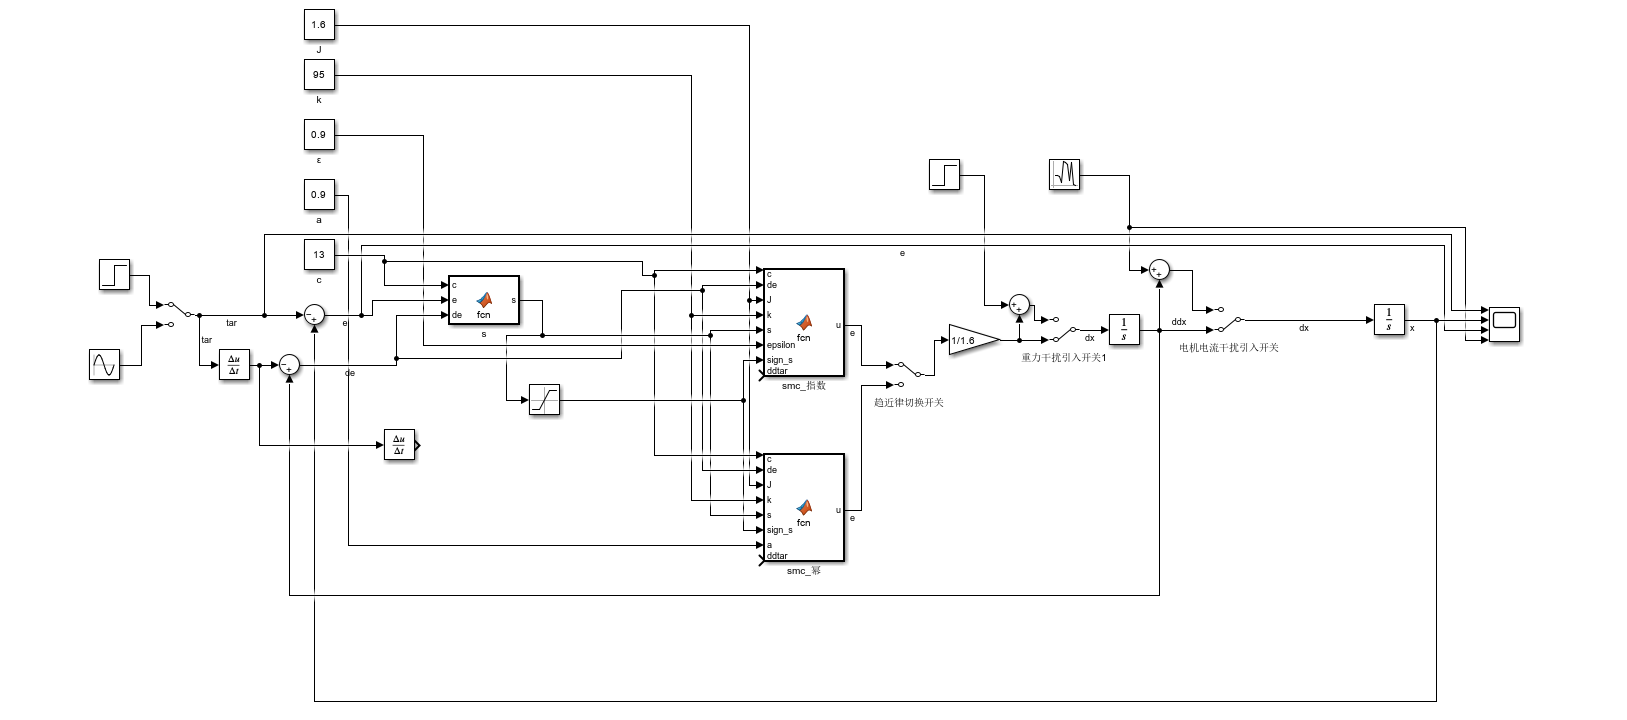
\includegraphics[width=0.9\textwidth]{../other/Yaw_1.png}
            \caption{左上Yaw控制器}

            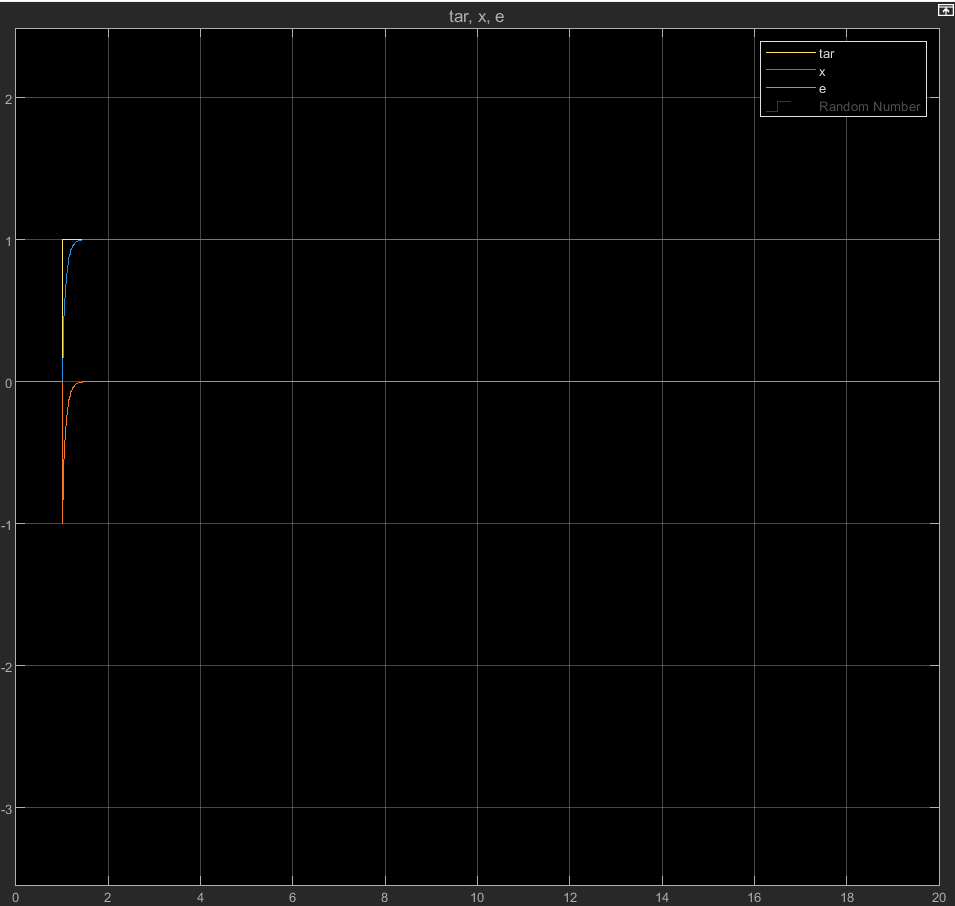
\includegraphics[width=0.7\textwidth]{../other/Yaw_11.png}
            \caption{左上Yaw控制器控制效果}
        \end{figure}
    \newpage

    \subsection{$\ddot{\theta_d}$ 问题}
    在仿真中,加入 $\ddot{\theta_d}$ 后会导致阶跃响应瞬间激发出一个较大的反方向的控制量,具体原因可能与仿真器及建模太过理想化导致,且在代码中加入该项后会导致抖震现象加重,但是影响并不剧烈,也对控制效果无明显提升,此处可能需要大家根据自己的机器结构尝试后,根据效果考虑选用哪一种,代码中两者均含有,只是含有该项的控制律注释掉了。
        \begin{figure}[htbp]
            \centering
            \begin{minipage}[t]{0.48\textwidth}
                \centering
                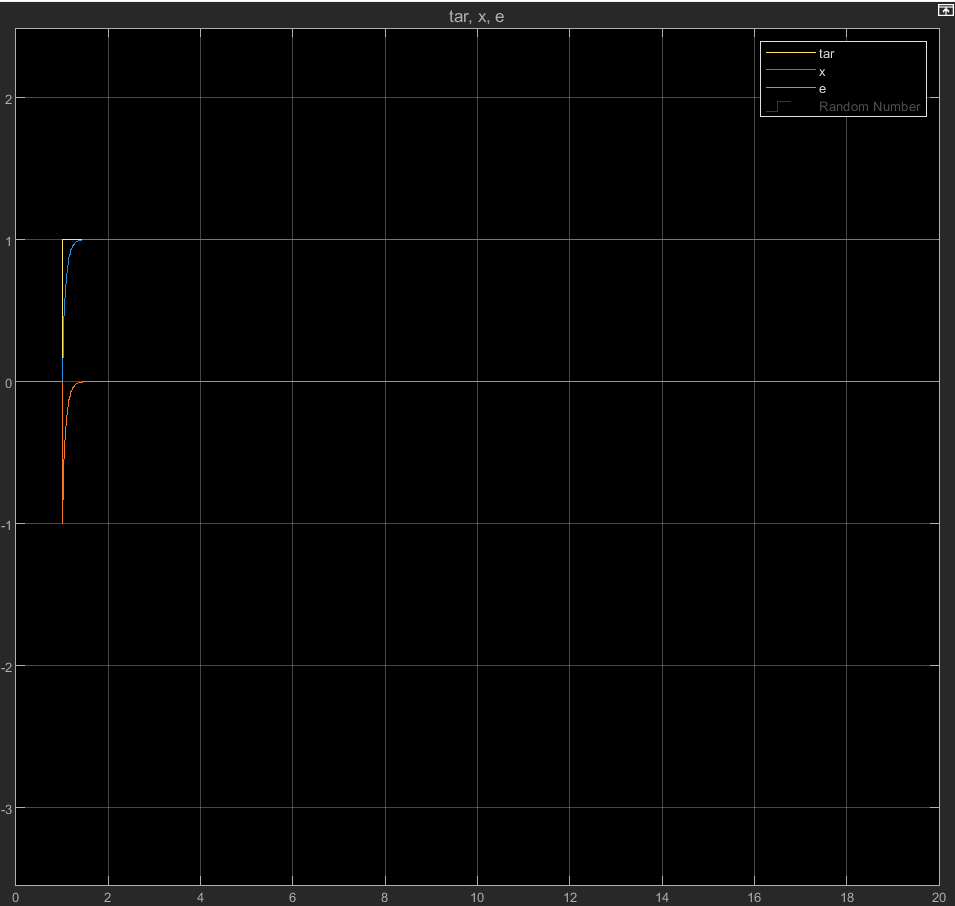
\includegraphics[width=\textwidth]{../other/Yaw_11.png}
                \caption{无 $\ddot{\theta_d}$}
                \end{minipage}
                \hfill
                \begin{minipage}[t]{0.48\textwidth}
                \centering
                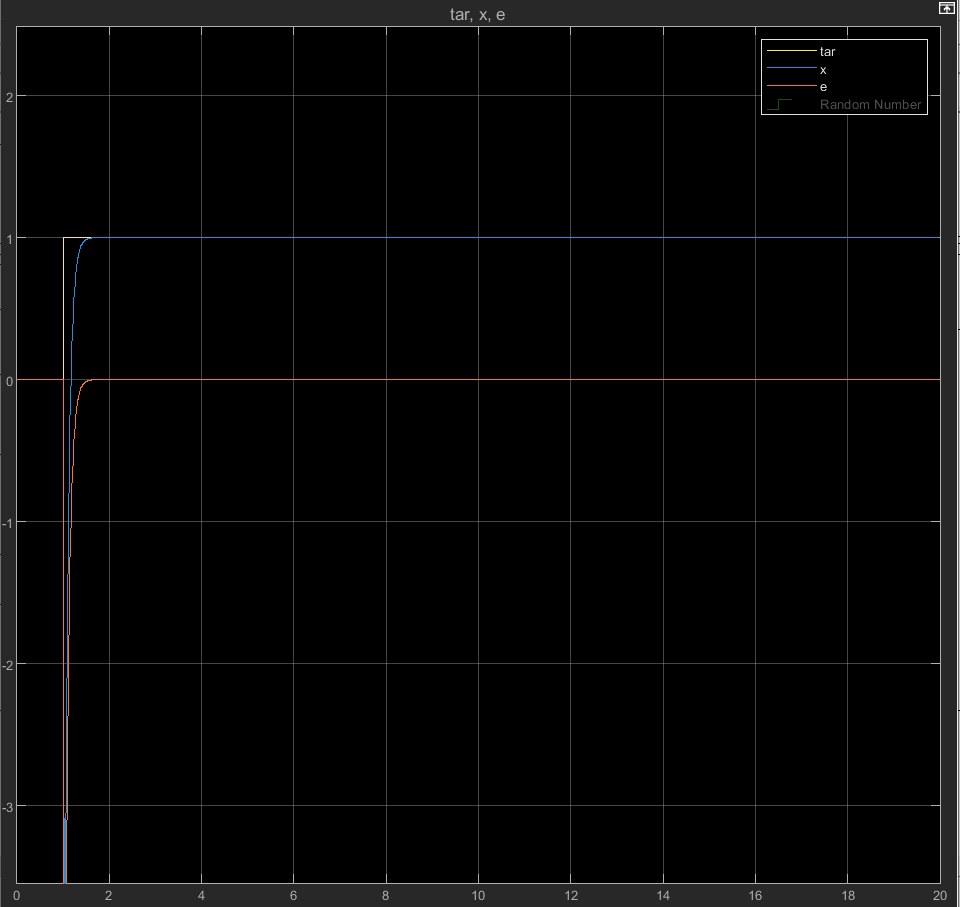
\includegraphics[width=\textwidth]{../other/Yaw_12.png}
                \caption{有 $\ddot{\theta_d}$}
                \end{minipage}
        \end{figure}
    \newpage

    \subsection{Pitch 控制器效果对比}
    下图中左边可以明显看到,在重力影响下,控制效果会一致保持有一个恒定值的稳态误差,而右图中可以看到,在重力影响下该稳态误差会收敛最终至 0。但是由于引入更多变量,调参难度会稍大些。(ps:为看的比较明显故将参数调至超调较明显的情况,实际应用可达到比此处更好的控制效果)
    \begin{figure}[htbp]
        \centering
        \begin{minipage}[t]{0.48\textwidth}
            \centering
            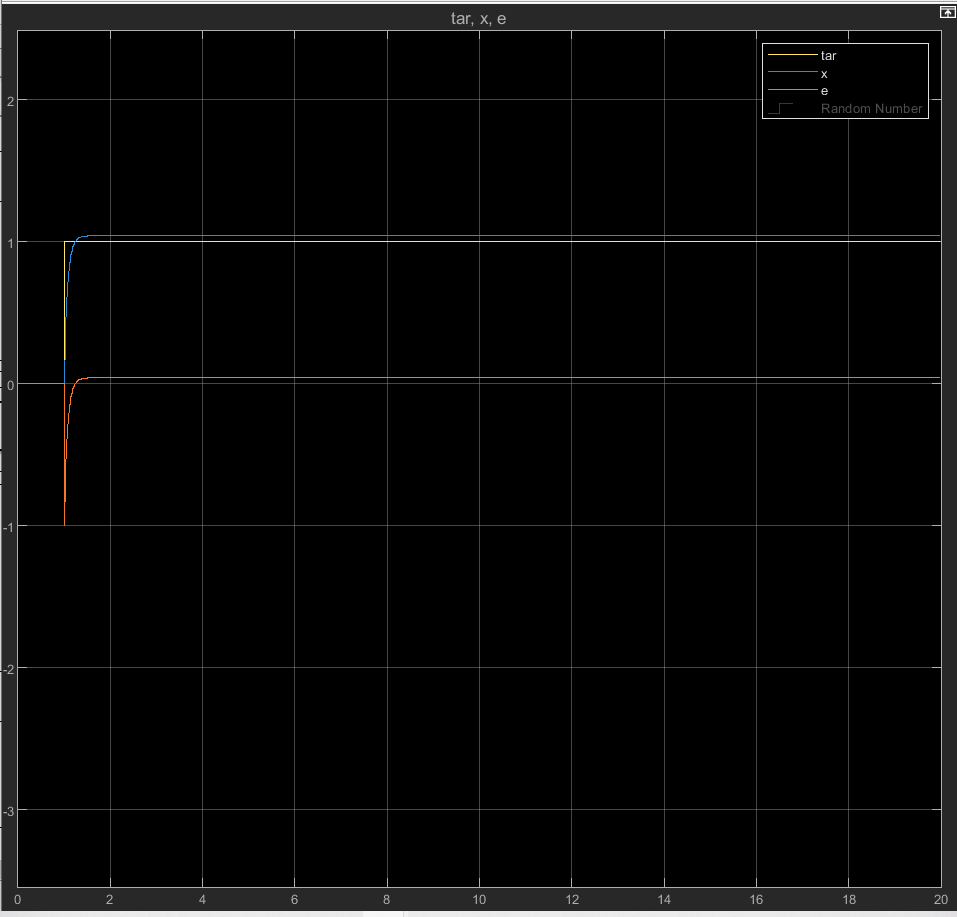
\includegraphics[width=\textwidth]{../other/Yaw_13.png}
            \caption{原控制器在重力干扰下效果}
            \end{minipage}
            \hfill
            \begin{minipage}[t]{0.48\textwidth}
            \centering
            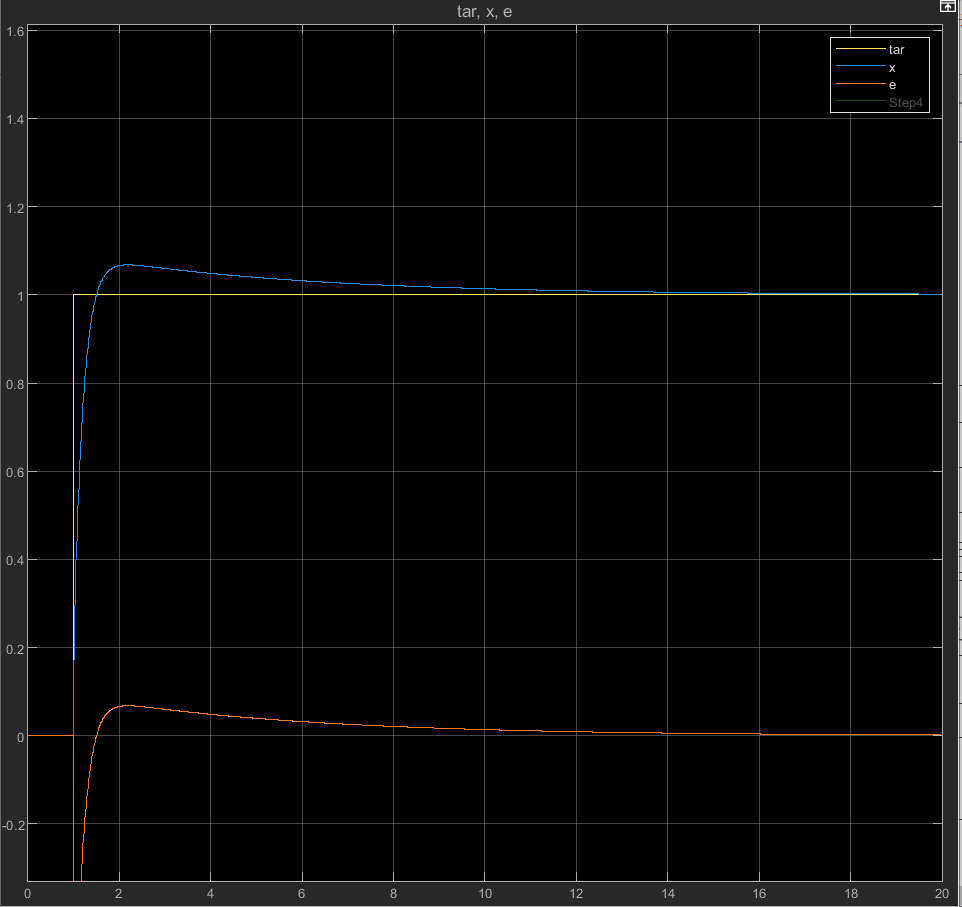
\includegraphics[width=\textwidth]{../other/Pitch_1}
            \caption{改进Pitch控制器在重力干扰下效果}
            \end{minipage}
    \end{figure}

\section{调参经验简单说两句}
$\varepsilon$ 为干扰绝对值上限,对效果影响不大。
\par
J 为转动惯量,可以找机械哥获取后微调。
\par
k 值太大会导致高频抖震,c 值太大会出现大幅度缓慢震荡。提高 k 值可减小超调并且提高响应速度,提高 c 值也可提高响应速度,但会导致超调加重,需平衡两者影响。Pitch 中,$c_2$ 与 $c_1$ 相比会小很多。这些均为个人经验,可能会对不同结构机器有些出入。
\par
死亡后要清除Pitch和速度控制中的积分变量值,否则会导致其持续累积而引起Pitch卡死及超射速问题!

\section{总结与展望}
(1)本控制器设计过程中,对电机的建模太过理想化,可采用系统辨识获取电机传递函数以更精细化控制器设计。
\par
(2)仿真设计也太过理想化,整个系统为连续信号贯穿始终,虽足以验证控制效果,但是仍与实际有较大差距,可构建离散信号建模以贴合实际。
\par
(3)该控制器为一阶滑模控制器,可优化为更高阶滑模控制器以根除抖震问题并提高控制效果与抗扰性能。

\newpage
\section{参考文献}
\begin{thebibliography}{99}

    \bibitem{liu2015}
    刘金琨. \textit{先进控制系统设计方法 (第3版)}. 国防工业出版社, 2015.
    
    \bibitem{csdn1}
    昔时扬尘处. 滑模变结构控制SMC(一)——滑模变结构控制的设计步骤 [EB/OL]. 
    \url{https://blog.csdn.net/qq_42249050/article/details/107224303}, 2020.
    
    \bibitem{zhihu1}
    Chenglin Li. 非线性系统(十三)滑模控制解析 [EB/OL]. 
    \url{https://zhuanlan.zhihu.com/p/138860110}, 2020.
    
    \bibitem{zhihu2}
    Y-box. 滑模控制器最强解析 [EB/OL]. 
    \url{https://zhuanlan.zhihu.com/p/78549442}, 2019.
    
    \bibitem{zhihu3}
    HuangTL. 滑模变结构控制 [EB/OL]. 
    \url{https://zhuanlan.zhihu.com/p/386592978}, 2021.
    
    \bibitem{zhihu4}
    纯狐. 现代控制理论—非线性鲁棒控制器\_sliding mode\_滑模控制 [EB/OL]. 
    \url{https://zhuanlan.zhihu.com/p/657512536}, 2023.
    
    \bibitem{csdn2}
    Neil motor. 永磁同步电机控制算法--改进指数趋近律滑模速度控制器 [EB/OL]. 
    \url{https://blog.csdn.net/m0_45796409/article/details/144173934}, 2024.
    
    \bibitem{zhihu5}
    半年这么快过去了. 滑模控制的一种简单理解 [EB/OL]. 
    \url{https://www.zhihu.com/tardis/zm/art/463230163?source_id=1005}, 2024.
    
    \end{thebibliography}


\end{document}